%%% template.tex
%%%
%%% This LaTeX source document can be used as the basis for your technical
%%% paper or abstract. Intentionally stripped of annotation, the parameters
%%% and commands should be adjusted for your particular paper - title, 
%%% author, article DOI, etc.
%%% The accompanying ``template.annotated.tex'' provides copious annotation
%%% for the commands and parameters found in the source document. (The code
%%% is identical in ``template.tex'' and ``template.annotated.tex.'')

\documentclass[conference]{acmsiggraph}

\TOGonlineid{45678}
\TOGvolume{0}
\TOGnumber{0}
\TOGarticleDOI{1111111.2222222}
\TOGprojectURL{}
\TOGvideoURL{}
\TOGdataURL{}
\TOGcodeURL{}

\title{Walk Motion Control in Partial Immersion}

\author{Samuel Carensac\thanks{e-mail:samuel.carensac@gmail.com}, Nicolas Pronost, Saida Bouakaz\\University Lyon 1, LIRIS}
\pdfauthor{Samuel Carensac}

\keywords{ Virtual Human, Physics based animation,  Motion control, Real-time liquid interaction, Offline optimization }

\begin{document}

\teaser{
   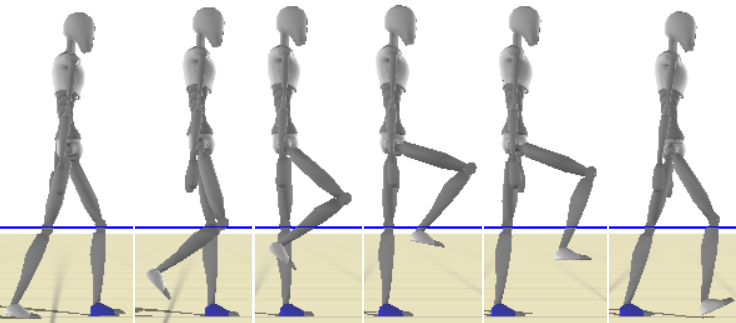
\includegraphics[height=1.5in]{images/3_6_1_50cm.png}
   \caption{Real-time physics-based simulation of walking of partially immersed bipeds. The method provides robust balance, adaptative gait style to character conditions and precise speed tracking. ***Not final image (need longer series)***}
\label{fig:intro}
}

\maketitle

\begin{abstract}

Physics-based animation is an increasingly studied subject because it allows more natural interactions with the virtual environment. Though some existing motion controllers can handle the simulation of interactions between a character and a liquid, only few focus on the simulation of the locomotion of immersed bipeds. In this paper we present a control strategy capable of simulating partially immersed character gait. The impact of the liquid on the motion is modeled through simple hydrodynamics. Our controller allows the combination of multiples gaits, the conservation of balance through intelligent foot placement and precise control of the character's speed. We determined the optimal parameters for the controller by using an optimization process. This optimization has been repeated for repeated for several scenarios where the character has to walk across a volume of liquid parametrized by its height. 
Finally our controller is capable of online adaptation to the variation of liquid height, to the modification of the liquid density and to the variation of the required character speed.

\end{abstract}

%\begin{CRcatlist}
%  \CRcat{I.3.3}{Computer Graphics}{Three-Dimensional Graphics and Realism}{Display Algorithms}
%  \CRcat{I.3.7}{Computer Graphics}{Three-Dimensional Graphics and Realism}{Radiosity};
%\end{CRcatlist}

\keywordlist

%% Use this only if you're preparing a technical paper to be published in the 
%% ACM 'Transactions on Graphics' journal.

%\TOGlinkslist

%% Required for all content. 

\copyrightspace

\section{Introduction}

Simulating realistic human motion is a key step in creating a virtual environment. Over the years, the simulated environments have become increasingly diverse and there are now complex environments with large numbers of elements that can influence the motion of the character. In those cases physics-based animation are chosen over kinematic animation since it doesn't need a series of exact position for each possible interaction. With virtual worlds becoming more complex it is now difficult to achieve realistic interactions between animated characters and the environment using kinematic animation methods. Physics-based animation uses physical phenomena (forces and torques) to manipulate the character. This allows the creation of a motion that will be directly impacted by the environment. A growing number of contributions are now working on building physics-based controllers \cite{geijtenbeek2012interactive}. Although they inherently allow obtaining interactions with the environment, the manipulation of the character becomes more complex as no direct control over the position of limbs of animated characters is possible.

The main challenge of a controller is to allow high level parameterization of the system. For example these parameters may be the speed, the direction of motion or the motion style. The need to simulate a large number of motion styles (walking, running, jumping...) makes creating a generic controller extremely challenging. Similarly, the mastery of multiples interactions with the environment also increases considerably the complexity of the system. This is why the existing controllers focus on the study of a limited number of motion styles and interactions with the environment \cite{geijtenbeek2012interactive}. This paper focuses on the control of walking in partial immersion conditions in a liquid. Our scientific objective is to define and implement the necessary mechanisms to a physics-based controller to allow real-time animation of a virtual character interacting with a liquid controlled by reference poses, a desired velocity and a heading. Our controller is also capable of great freedom of gait and precise tracking of the character's motion speed.

This paper will start by presenting the existing works related to our contribution (section  \ref{sec:previous_works}). Section \ref{sec:overview} proposes a global view of our system followed by a detailled description of each components in the sections \ref{sec:ext_forces} and \ref{sec:control_framework}. We present our results in section \ref{sec:results} and discuss the limits of our controller in a short conclusion (section \ref{sec:conclusion}).
 
\section{Previous works}
\label{sec:previous_works}

Numerous works about control of character with physics based simulation can be found in the literature \cite{geijtenbeek2012interactive}. Among those works some share common characteristics with our objectives.

Our work share some features of the SIMBICON (SIMple BIped CONtroler) \cite{yin2007simbicon} and recent related works. Among them \cite{coros2009robust} propose a system integrating multiples controllers for navigation task. The drawback is that the system is designed to use optimization to determine how the different controllers should be used. To enable the use of low gains in the PD-controlers different methods have been used such as a feedforward system\cite{yin2007simbicon} or the computation of torques to compensate the effect of gravity \cite{coros2010generalized}.

\textbf{\textit{Balance control}} is one of the key systems in physics based simulation. The original SIMBICON uses secondary PD-controllers on the key joints (stance ankle and swing hip) to dynamically adapt the tracked positions. One way to compute a balance aware foot placement during walk motion is to use an Inverted Pendulum Model (IPM) \cite{coros2010generalized,kajita20013d}. The IPM can be used to dynamically compute the trajectory of the swing foot but it limits the range of possible gaits styles.

\textbf{\textit{Velocity control}} is often one of the required characteristics of physics based controllers.  Some works propose systems capable of adapting to online variations of the desired velocity. \cite{coros2009robust} obtains it by combining multiples controllers for specific motions (walk forward, walk backward …). The IPM based systems offers an inherent, though imprecise as it doesn't consider the observed velocity, control\cite{coros2010generalized}. The use of horizontal virtual forces has been a way to obtain a precise control of the speed and balance of the character \cite{coros2010generalized,geijtenbeek2012simple}. This system is based on secondary PD-controllers to compute the necessary force. The static gains and constant used in those systems make them unable to track correctly the desired speed when the character is subject to a variable environment (e.g. apparition of a liquid medium). 

\textbf{\textit{Movement in liquids}} have been studied in both simulation \cite{yang2004layered,si2014realistic} and biomechanics \cite{barela2006biomechanical,chevutschi2009comparison}. Those works mainly focus on swimming control for simulation works and walk study with high level of immersion for biomechanics studies making them unusable for our scenarios. Other approaches worked on simulating human walk under wind forces \cite{lentine2011creature}. Most of those works use Navier-Stockes equations to simulate the liquids making them unable to obtain real-time and interactive simulations.

 In this paper we propose a new controller showing the following caracteristics:
\begin{itemize}
\item{real-time interactive simulation by using simple hydrodinamics to simulate the impact of the liquid}
\item{dynamic gait style adaptation by combining multiples reference controllers}
\item{liquid impact aware gait styles by specific IPM usage and offline optimisation}
\item{precise tracking of desired velocity by using learning strategies}
\end{itemize}

\section{Overview}
\label{sec:overview}

\begin{figure}[t]
\centering
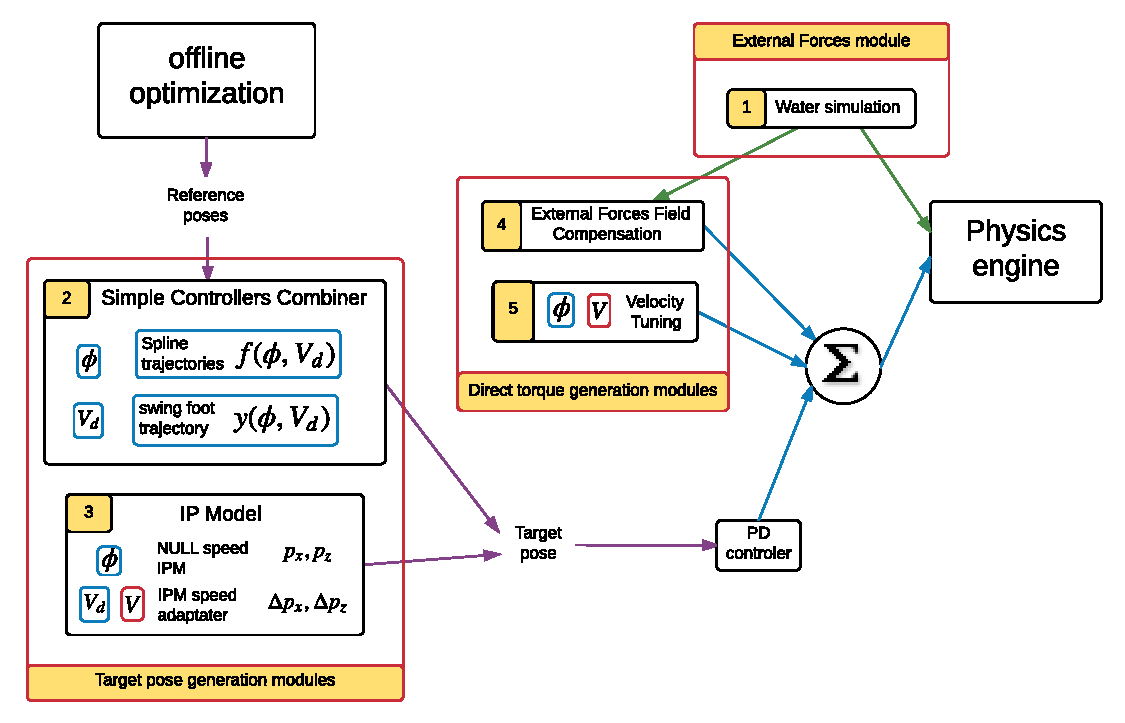
\includegraphics[scale=0.45]{images/general_process.pdf}
\caption{System Overview. The key components of the system are: (1) influence of liquid through external forces; (2) a combination of simple controllers generating the target poses; (3) an IPM for predictive foot placement; (4) an external force fields compensation helping the PD-controller; (5) velocity tuning for fine velocity and balance corrections.}
\label{fig:shema_controler}
\end{figure}

Our controller consists of five key components that are classified in three categories (figure \ref{fig:shema_controler}).

We start by simulating the liquid impact on the character by applying external forces computed by simple hydrodynamics (drag, friction and buoyancy) allowing us to obtain real-time interactions between the liquid and the character (section \ref{sec:ext_forces}).
We use a combination of various controllers each one defining a gait style depending on character condition (e.g. liquid level, desired speed) allowing an adaptive evolution of the gait style (section \ref{sec:multi_state}). The specified trajectories for the joints composing the swing leg are overridden by the results of an IPM if the character is in the falling phase of a step or if the controller detects a loss of balance (section \ref{sec:specific_ipm}).

We augment the PD-controller with torques computed through an external force-field compensation. This system is a generalization of \cite{coros2010generalized} gravity compensation and help us compute a significant part of the necessary torques (section \ref{sec:ext_force_comp}).

Our controller presents a precise tracking of the desired velocity through an adaptive offset on the swing foot position computed by the IPM (section \ref{sec:ipm_alt}). We also propose an amelioration of \cite{coros2010generalized} fine-scale control by considering the intra-step speed variation of the character to compute a more efficient virtual force  (section \ref{sec:speed_virt_force}).

Finaly, we use an offline optimisation to generate the references poses used by the Simple Controllers Combinator defining a gait style specific to interactions with liquids (section \ref{sec:optimisation}).


\section{External Forces}
\label{sec:ext_forces}

The only external forces generated by our model are the forces used to simulate the impact of the liquid on the character.
To compute them we use simple hydrodynamics. We consider two types of forces. The first one is the buoyancy. We use the well-known equation $F_{B}=-V_i \rho g$ with $V_i$ the immersed volume of the physics representation of the character.
The second type of forces is the parasitic drag. We restrict the considered physics phenomena to the form drag and the skin friction. Also we simplify the computation of the resulting force $F_D$ by using the following equation:
$$
F_D=\frac{1}{2} \rho v^2 A_n C_d \times \mu
$$
With \(C_d\) the drag coefficient, \(\rho\) the fluid density, \(A_n\) the cross sectionnal area and \(v\) the relative speed to the fluid. Due to the complexity of dynamically computing $C_d$ we fix it to 1.0 (average value for a man). $\mu$ is a simple coefficient representing the fluid viscosity allowing us a rough representation of the friction. The velocity varying through the limbs we use a finite elements decomposition of the surface of each limb and compute the parasitic drag for each element.


\section{Control Framework}
\label{sec:control_framework}

Our system is built on the version of SIMBICON presented by \cite{coros2010generalized}. The trajectories for the ankles, pelvis, back and head are specified in the coordinates system of the character. This coordinate system is similar to the global one but the z axis indicates the direction that the character is currently facing. The trajectories for the shoulders, elbows, toes and the knee of the stance leg are specified using each joint local coordinates.
Unlike \cite{coros2010generalized} we allow manual specification of the swing foot trajectory. This specification is made in the coordinates system relative to the swing hip.

\subsection{Simple Controllers Combiner}
\label{sec:multi_state}

The \textit{Simple Controllers Combiner} allows us to observe dynamic variations of the gait style depending on the conditions of the character (e.g. liquid level). The principle is to use multiples simple controllers that are specified for one set of conditions. For this work we limit the conditions to the walking speed and the liquid level but the system could handle way more complex specifications. Each simple controller defines the trajectories for the joints that present significant variations from one standard controller. For example our standard controller is a forward walk controller and as such it specifies that the heel hits the ground before the toes do. If we want to be able to walk backward we will have to specify a simple controller specifying that the toes hit the ground before the heel and affect it to a negative sagittal speed. Our system diverge from the one presented by \cite{coros2009robust} by two characteristics. First, we don't require each individual controller to produce a stable motion. In our system the balance is acquired by the use of an IPM. Second, each individual controller only specifies the joints where the variation from the standard state is significant. On a more conceptual view our system differs by the fact that we just want to specify the variations of the gait and not the variations of control strategy. Also we don't require an optimization step to find the optimal combination of the simple controllers. When the character ends a step, the system will compute a new trajectory for each joint. To find those trajectories we use an interpolation following a square-law between the trajectories specified for the two nearest simple controllers. For example, if we use controllers defined only by their reference speeds, we will use the two controllers $f_1$ and $f_2$ defined for the speeds $V_1$ and $V_2$ that are the nearest from the desired speed $V_d$ respecting $V_1 < V_d < V_2$. If we can't find two speed respecting this rule we directly use the nearest simple controller. The following equation details how the resulting trajectories $f$ are computed:
$$
f(\phi)=f_1(\phi)*(1-R)+f_2(\phi)*R   \quad \textrm{with} \quad   R=(\frac{V_d-V_1}{V_2-V_1})^2
$$

\subsection{Inversed Pendulum Model}
\label{sec:IPM}

We use an \textit{Inversed Pendulum Model} (IPM) suposing constant leg size and zero desired velocity similar to the one used by \cite{coros2010generalized}. We have modified this IPM to allow the specification of previously impossible gaits styles and to enable a better tracking of the user's desired velocity. 

\subsubsection{Specific IPM Usage}
\label{sec:specific_ipm}

Our idea to enable the specification of new gait is that the IPM doesn't need to control the swing foot during the whole step. We only need to control the position of the swing foot when the character is in a falling state, meaning when the vertical speed of the center of mass is positive $V_{COM}>0$. During a step, the falling phase corresponds to the end of the step. So during the first part of the step we will use a user defined trajectory for the swing foot. This allows the observation of vertical movement of the swing foot without any horizontal movement, which was previously impossible. This kind of gait style is important in our case because it is typical of a character trying to minimize the opposition of the liquid (Figure \ref{fig:intro}).



\subsubsection{IPM Result alteration}
\label{sec:ipm_alt}


The major flaw of the simple linear modification of IPM result depending on the desired character velocity used by \cite{coros2010generalized} is that it only function properly near the velocity for which the linear factor used has been optimized. In particular, this system cannot handle the transition from constrained environment like the presence of a fluid medium to an unconstrained one. Our solution is to add a supplementary offset $\Delta(x,z)$ to the results of the IPM. This new offset will be adapted at the end of each step depending on the difference between the current character velocity and the desired velocity $\Delta(x,z) = \Delta(x,z)+\beta(V-V_d)$ with $\beta$ a positive constant. So the swing foot position $P(x,z)$ we will use when considering the results of the IPM $P_{IPM}(x,z)$ will be:
$$
P(x,z) = P_{IPM}(x,z) - \alpha V_d + \Delta(x,z)
$$ 

\subsection{External Forces Fields Compensator}
\label{sec:ext_force_comp}

Our \textit{ External Forces Fields Compensator} is an extension of the gravity compensation proposed by \cite{coros2010generalized}. The goal is to dynamically compute a part of the necessary torques at each joint thus permitting the use of lower gains in the main PD-controller. The external forces that we consider are the weight $P=mg$ of each part of the character and the buoyancy $F_B=-\rho V_i$. We chose to ignore the liquid drag because its calculation implies the uses of a lot of small forces (depending on the precision of the finite elements) which cannot be simplified as on global force for each limb, meaning it would be time consuming to compensate it. So the final virtual force applied to each body part is:
$$
F=-mg+\rho V_i
$$


\subsection{Velocity Tuning}
\label{sec:speed_virt_force}

\begin{figure*}[t]
\centering
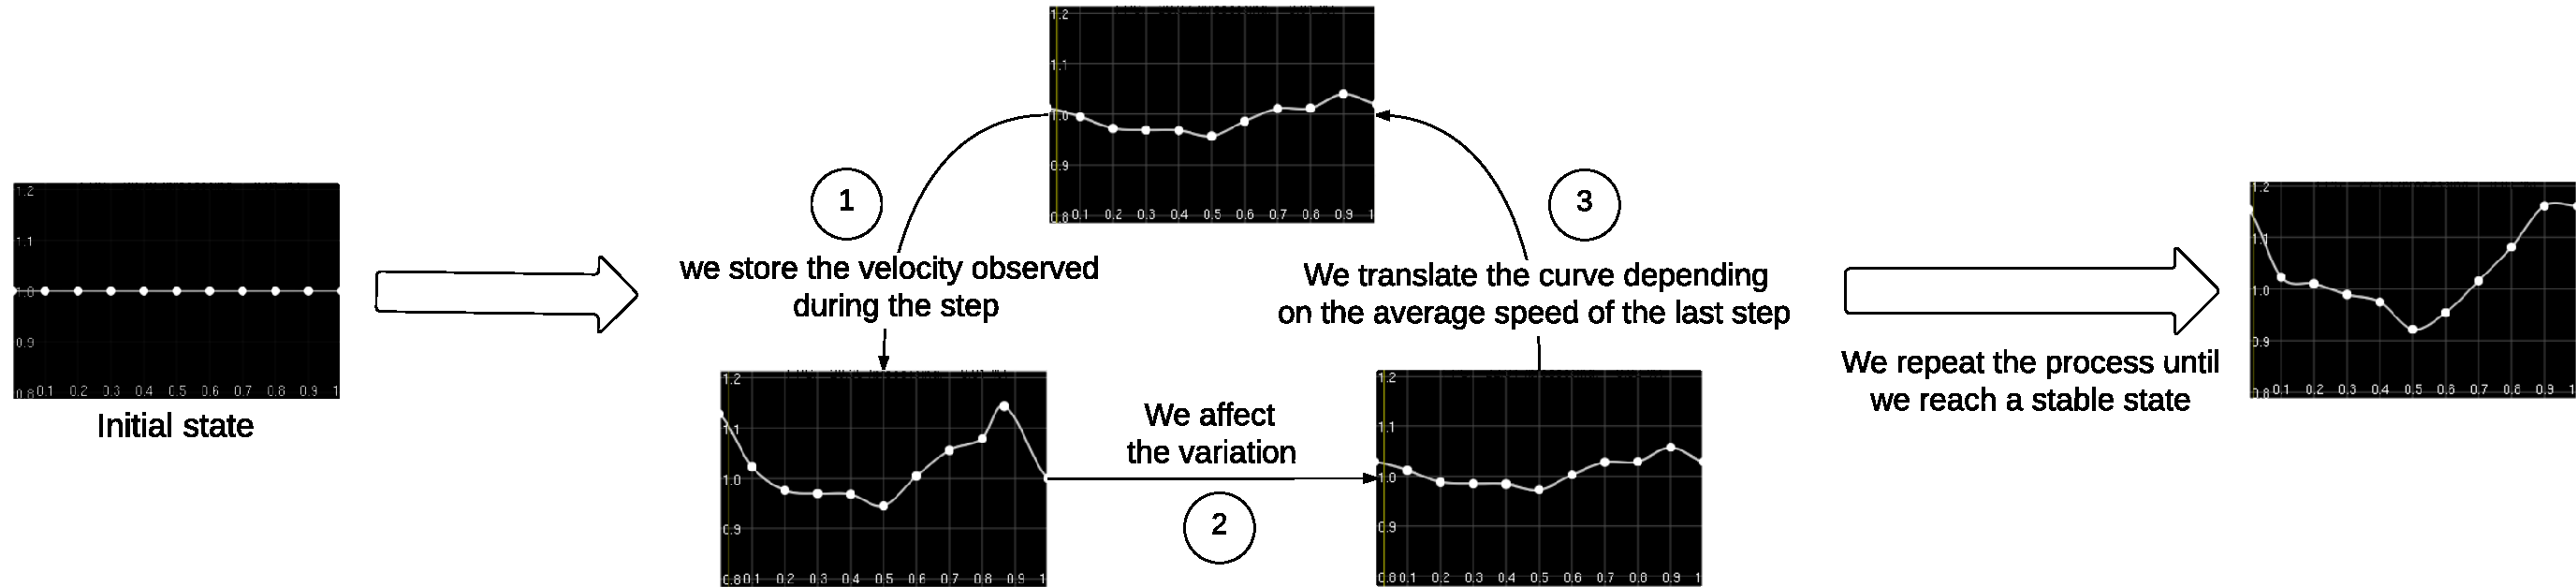
\includegraphics[scale=0.45]{images/speed_curve_learner.pdf}
\caption{Process of learning the adapted required velicity curve}
\label{fig:speed_curve_learner}
\end{figure*}


Similarly to \cite{coros2010generalized} velocity tuning, ours applies a horizontal virtual force to obtain a fine control of the speed and balance. Our version presents three differences from \cite{coros2010generalized}'s system. First we don't consider the same chain of limbs. Instead of considering one chain that goes from the head to the stance foot we use two: one going from the pelvis to the stance foot and one consisting of the torso alone. This modification comes from two things. First, we don't consider the head in the top chain because we don't want the character to tilt the head to control its velocity. Second, we separate the torso from the lower body because we estimate that the main control strategy of the speed should be to simply tilt the torso and not to exert huge torques on the stance ankle. Our jacobian considers the mass $M_i$ of each individual limb:
$$
J_n ^T (p)=\frac{1}{M}\sum_{\substack{0<i\leq n}} ((P_i(x,y,z)-P_{i-1}(x,y,z))*M_i)
$$

 With \(M\) the sum of every limbs considered by the velocity tuning \(P_i(x,y,z)\) the position of the \(i\) joint and \(P_0(x,y,z)\) the application point of the virtual force. This modification allows us to give more impact to the joints controlling a lot of mass (i.e. joint between the pelvis and the torso). Finally we will consider the intra-step variations of velocity. In most cases, the velocity during a step is not constant. Supposing it constant like \cite{coros2010generalized} may cause the apparition of undesired behavior asking the character to slow at the start of the step, then accelerate when near the middle of the step to slow once again near the foot strike. This is why we use a system learning the curve defining the different velocities we need to ask the controller during a step to result in a somewhat constant virtual force. This system is based on an iterative principle. During the step we record the observed velocities for the center of mass. When the step ends, if the average variation between the learning curve and the observed one is lower than a threshold, we adapt our learning curve so that its figure fits the figure of the observed speed curve. Then we adapt our learning curve depending on the ratio between the desired velocity and the average observed velocity $R=V_d/V_{avg}$ (see figure \ref{fig:speed_curve_learner}). If the variation is higher than the threshold it means the character is not in a stable motion anymore. In that case we stop adapting our learning curve and switch to the use of recovery steps, meaning the full trajectory of the swing foot will be defined by the IPM. We stay in recovery mode until the average variation between the observed speed and the specified one is lower than the threshold. If it takes more than five steps we reset the learning curve to a constant one with the desired velocity value and we start learning once again. Our system uses one learning curve for the sagittal speed and two curves of the coronal speed (one for each stance).

\subsection{Offline Optimisation}
\label{sec:optimisation}


\section{Results}
\label{sec:results}

Lorem ipsum dolor sit amet, consectetur adipisicing elit, sed do
eiusmod tempor incididunt ut labore et dolore magna aliqua. Ut enim ad
minim veniam, quis nostrud exercitation ullamco laboris nisi ut
aliquip ex ea commodo consequat. Duis aute irure dolor in
reprehenderit in voluptate velit esse cillum dolore eu fugiat nulla
pariatur. Excepteur sint occaecat cupidatat non proident, sunt in
culpa qui officia deserunt mollit anim id est laborum.


\section{Conclusion}
\label{sec:conclusion}

Lorem ipsum dolor sit amet, consectetur adipisicing elit, sed do
eiusmod tempor incididunt ut labore et dolore magna aliqua. Ut enim ad
minim veniam, quis nostrud exercitation ullamco laboris nisi ut
aliquip ex ea commodo consequat. Duis aute irure dolor in
reprehenderit in voluptate velit esse cillum dolore eu fugiat nulla
pariatur. Excepteur sint occaecat cupidatat non proident, sunt in
culpa qui officia deserunt mollit anim id est laborum.

\section*{Acknowledgements}

Lorem ipsum dolor sit amet, consectetur adipisicing elit, sed do
eiusmod tempor incididunt ut labore et dolore magna aliqua. Ut enim ad
minim veniam, quis nostrud exercitation ullamco laboris nisi ut
aliquip ex ea commodo consequat. Duis aute irure dolor in
reprehenderit in voluptate velit esse cillum dolore eu fugiat nulla
pariatur. Excepteur sint occaecat cupidatat non proident, sunt in
culpa qui officia deserunt mollit anim id est laborum.

\nocite{*}
\bibliographystyle{acmsiggraph}
\bibliography{template}
\end{document}
